\documentclass[12pt,a4paper,onecolumn]{article}
\usepackage[utf8]{inputenc}
\usepackage[T1]{fontenc}
\usepackage[french]{babel}

% ------------------------- Color table ----------------------------------------
\usepackage{multirow}
\usepackage[table]{xcolor}
\definecolor{maroon}{cmyk}{0,0.87,0.68,0.32}
% ------------------------------------------------------------------------------

\usepackage{amscd}
\usepackage{amsthm}
\usepackage{physics}
\usepackage[left=2.2cm,right=2.2cm,top=2cm,bottom=2cm]{geometry}
\usepackage{textcomp,gensymb} %pour le °C, et textcomp pour éviter les warning
\usepackage{graphicx} %pour les images
\usepackage{caption}
\usepackage{subcaption}
\usepackage[colorlinks=true,
	breaklinks=true,
	citecolor=blue,
	linkcolor=blue,
	urlcolor=blue]{hyperref} % pour insérer des liens
\usepackage{epstopdf} %converting to PDF
\usepackage[export]{adjustbox} %for large figures

\usepackage{array}
\usepackage{dsfont}% indicatrice : \mathds{1}


% -------------------------- Mathematics ---------------------------------------
\graphicspath{{images/}{../images/}} % For the images path
% ------------------------------------------------------------------------------

% -------------------------- Mathematics ---------------------------------------
\usepackage{mathrsfs, amsmath, amsfonts, amssymb}
\usepackage{bm}
\usepackage{mathtools}
\usepackage[Symbol]{upgreek} % For pi \uppi different from /pi
\newcommand{\R}{\mathbb{R}} % For Real space

% ------------------------------------------------------------------------------


% -------------------------- Code format ---------------------------------------
\usepackage[numbered,framed]{matlab-prettifier}
\lstset{
	style              = Matlab-editor,
	basicstyle         = \mlttfamily,
	escapechar         = '',
	mlshowsectionrules = true,
}
% ------------------------------------------------------------------------------

% ------------------------- Blbiographie --------------------------------------
% \usepackage[backend=biber, style=science]{biblatex}
% \addbibresource{biblio.bib}
% ------------------------------------------------------------------------------


\setcounter{tocdepth}{4} %Count paragraph
\setcounter{secnumdepth}{4} %Count paragraph
\usepackage{float}

\usepackage{graphicx} % for graphicspath
% \graphicspath{{../images/}}

\usepackage{array,tabularx}
\newcolumntype{L}[1]{>{\raggedright\let\newline\\\arraybackslash\hspace{0pt}}m{#1}}
\newcolumntype{C}[1]{>{\centering\let\newline\\\arraybackslash\hspace{0pt}}m{#1}}
\newcolumntype{R}[1]{>{\raggedleft\let\newline\\\arraybackslash\hspace{0pt}}m{#1}}

% to start counting section to 6


% ------------------------ General informations --------------------------------
\title{Math M2 Probabilistic graphical models 2017/2018}
\author{Vincent Matthys}
\graphicspath{{images/}}
% ------------------------------------------------------------------------------

\begin{document}
\begin{tabularx}{0.8\textwidth}{@{} l X r @{} }
	{\textsc{Master MVA}}       &  & \textsc{Rapport expérimental} \\
	\textsc{3D Computer Vision} &  & {Vincent Matthys}             \\
\end{tabularx}
\vspace{1.5cm}
\begin{center}
	\rule[11pt]{5cm}{0.5pt}

	\textbf{\LARGE \textsc{Détecteurs de coins d'Harris}}
	\vspace{0.5cm}\\
	Vincent Matthys\\
	\rule{5cm}{0.5pt}
	\vspace{1.5cm}
\end{center}

Ce projet consiste en un développement dans l'élaborateur d'un détecteur de coins d'Harris, ainsi que d'un rafinement des détections par \textit{adaptive non-maximal suppression}. Le rapport qui suit regroupe différentes observations quand à son utilisation sur différentes images, avec différents paramètres et dans des conditions différentes, ceci dans un soucis d'évaluation qualitative du progamme délivré.

\tableofcontents
\section{Différentes scènes}

En figure~\ref{fig_1} sont présentés 4 résultats donnés par le détecteurs de coins de Harris implémenté, sur des images de taille comparable, avec les paramètres suivants :
\begin{itemize}
	\item \( \sigma_d = 1\) écart-type du noyau de convolution pour la dérivation.
	\item \( \sigma_i = 1\) écart-type de la fenêtre gaussienne de lissage des images produits.
	\item \( \kappa = 0.05\) constante multiplicative de la fonction de réponse
	\item \( threshold = 0.01\) seuil global (en fonction de la réponse maximale) en deça duquel aucune réponse n'est considérée.
	\item \(local = 3\) délimite la fenêtre de recherche du maximum local
	\item \(c = 0.7\) seuillage au delà duquel le point est automatiquement détecté.
	\item \( b = 50\) nombre de détections souhaité.
\end{itemize}
\begin{figure}[H]
	\centering
	\begin{subfigure}[b]{\textwidth}
		\centering
		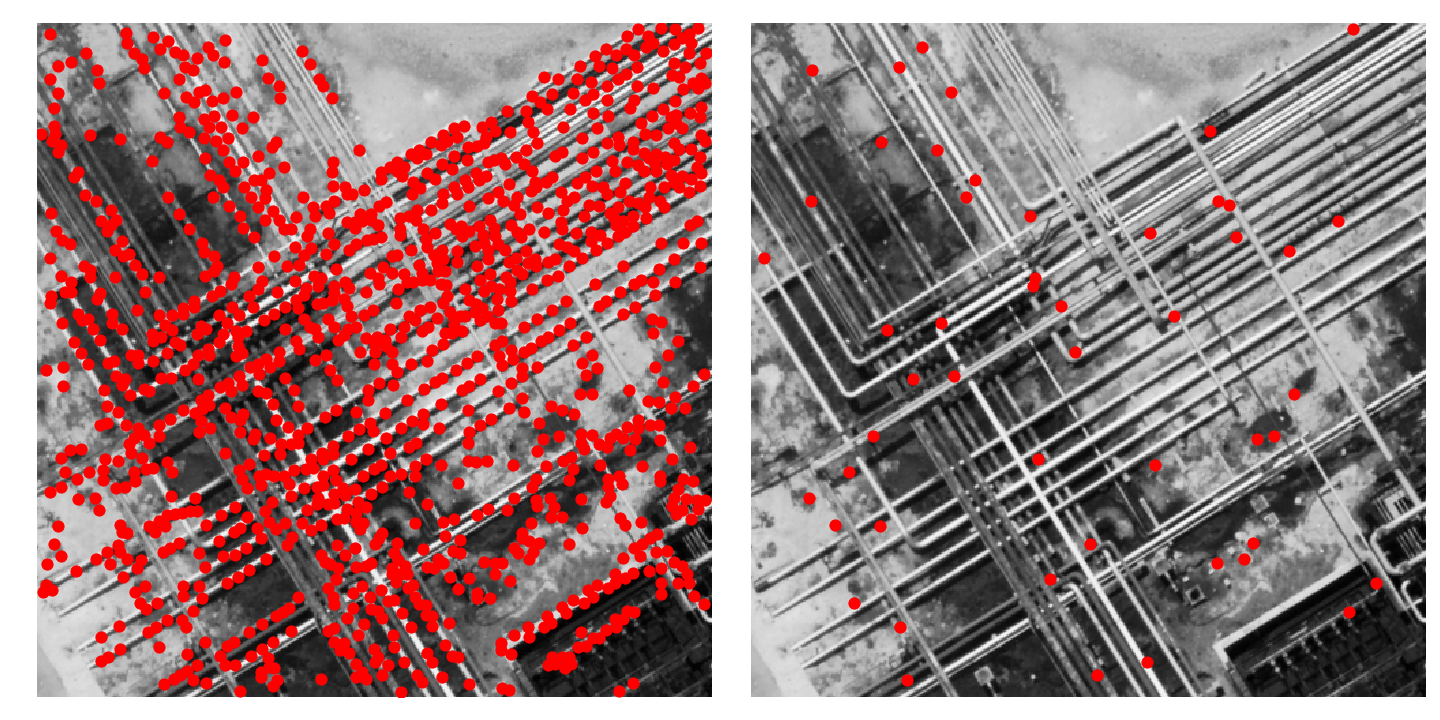
\includegraphics[height = 0.20\textheight]{1_bouc}
		\subcaption{Image Bouc, 495x495 pixels : 1265 coins détectés avant anms, 50 après}
		\label{fig_1_bouc}
	\end{subfigure}
	\begin{subfigure}[b]{\textwidth}
		\centering
		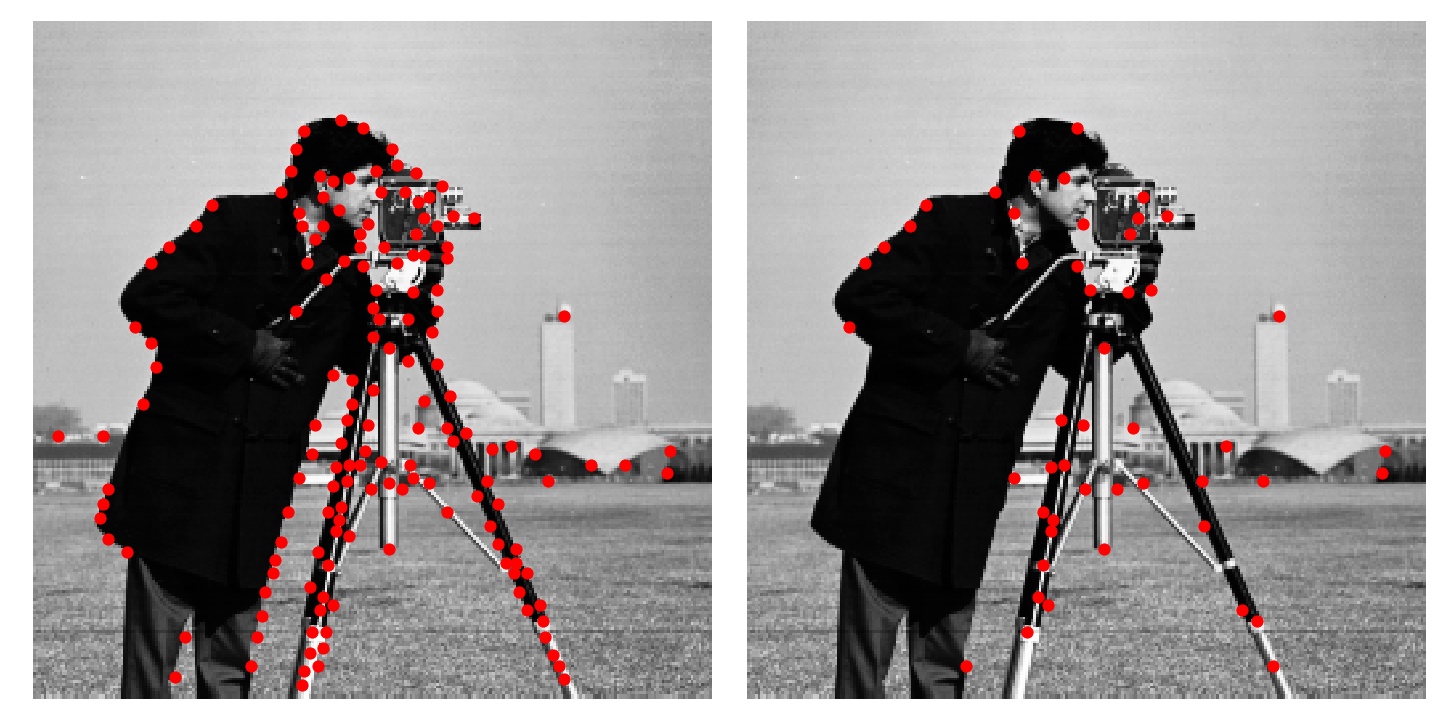
\includegraphics[height = 0.20\textheight]{1_cameraman}
		\subcaption{Image Cameraman, 256x256 pixels : 156 coins détectés avant anms, 50 après}
		\label{fig_1_cameraman}
	\end{subfigure}
	\begin{subfigure}[b]{\textwidth}
		\centering
		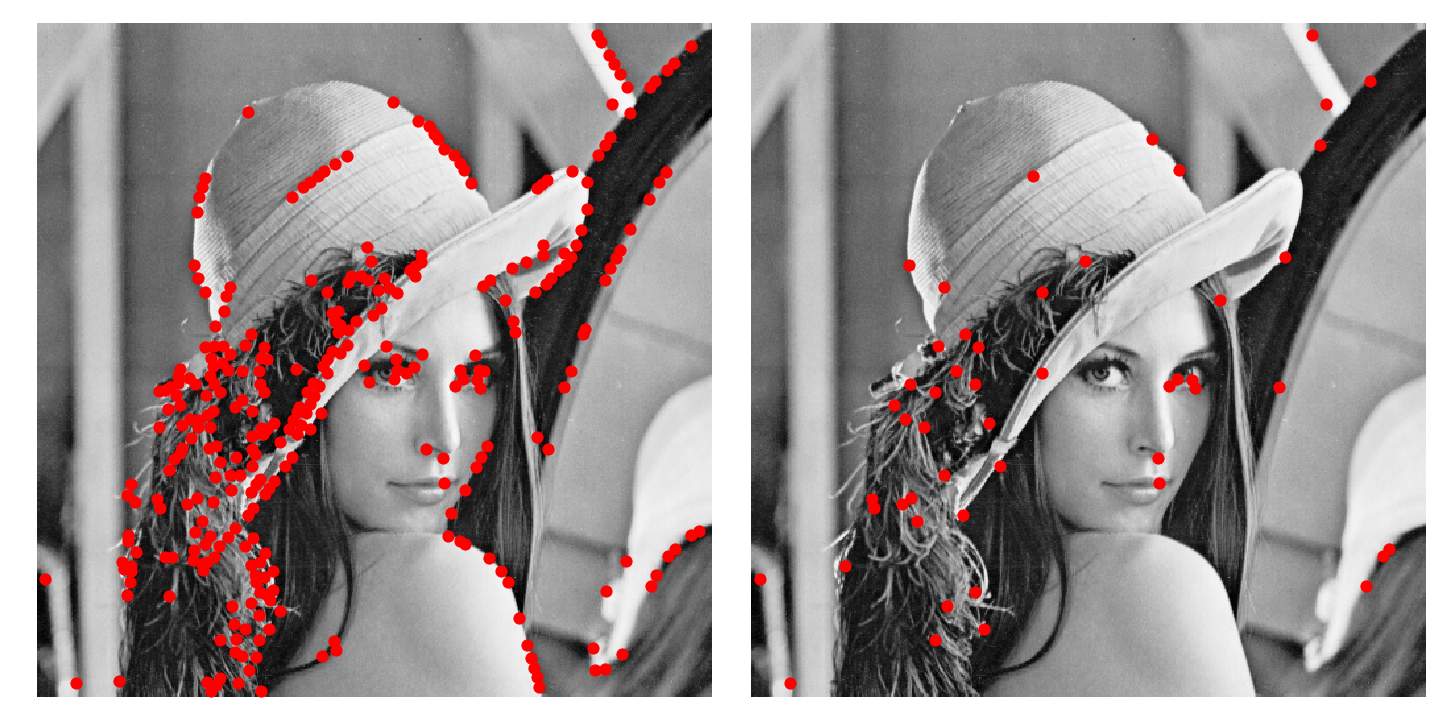
\includegraphics[height = 0.20\textheight]{1_lena}
		\subcaption{Image Lena, 512x512 pixels : 326 coins détectés avant anms, 50 après}
		\label{fig_1_lena}
	\end{subfigure}
	\begin{subfigure}[b]{\textwidth}
		\centering
		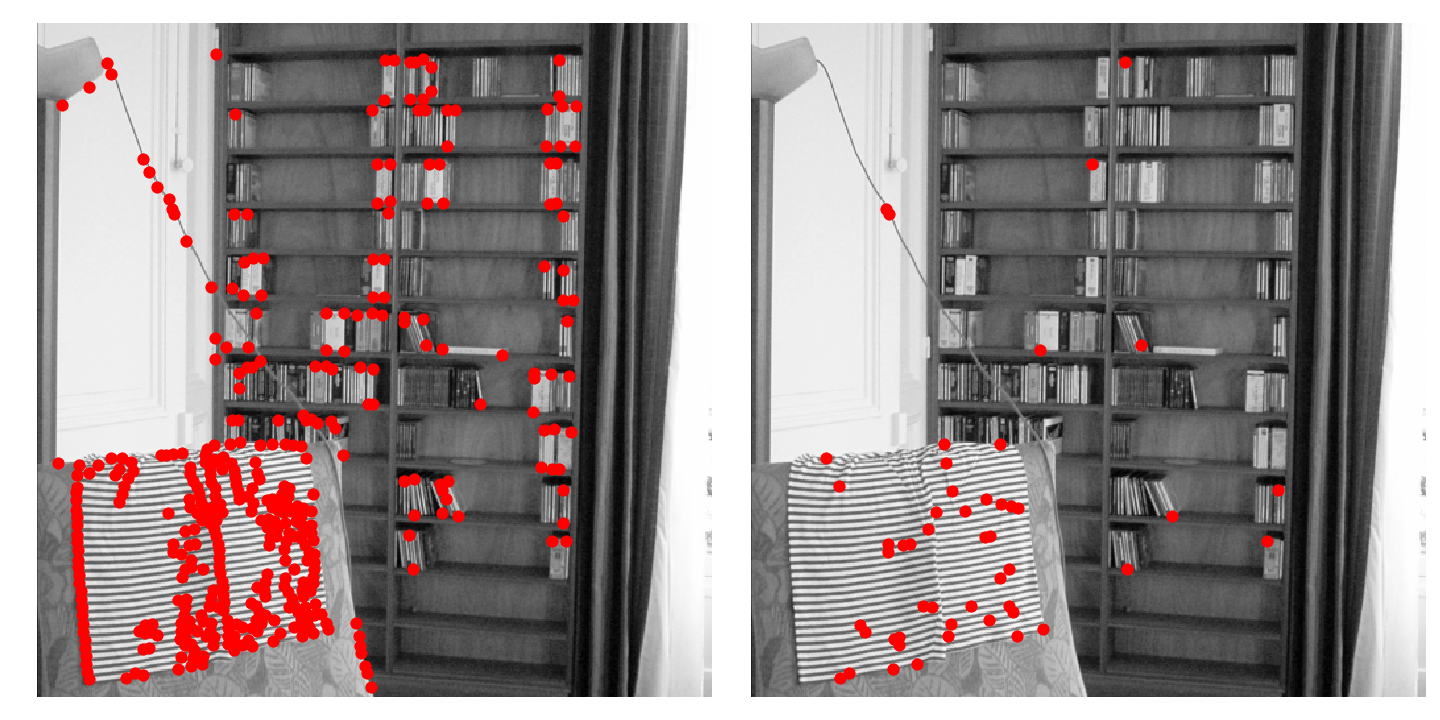
\includegraphics[height = 0.20\textheight]{1_room}
		\subcaption{Image Room, 512x512 pixels : 407 coins détectés avant anms, 50 après}
		\label{fig_1_room}
	\end{subfigure}
	\caption{Détecteurs de coins d'Harris sur différentes scènes. Colonne de gauche, sans \textit{adaptative non-maximal supression} ; colonne de droite, avec \textit{adaptative non-maximal supression}}
	\label{fig_1}
\end{figure}
En figure~\ref{fig_1_bouc}, on constate un très grand nombre de coins détectés, 5 fois supérieur aux autres images de même taille. Ceci est très bien expliqué par la géométrie du circuit représenté dans l'image, composé essentiellement de lignes ayant une forte réponse dans les images produits. Dans les 3 autres images~\ref{fig_1_cameraman}~\ref{fig_1_lena}~\ref{fig_1_room}, le nombre de coins détectés est sensiblement identique, si on le raméne à la taille de l'image. On constate légèrement plus de détections dans l'image Room pour les mêmes raisons que l'image Bouc, dans le carré de tissu présentant des lignes non totalement horizontales répondant fortement dans les images produits.

Une autre constatation importante est la localisation des détections, qui se situent dans les zones non constantes par morceaux, \textit{a fortiori} très constratées. Ceci est encore une fois expliqué par la réponse nulle de telles zones dans les images produits.

Enfin, l'\textit{adaptative non-maximal supression} agit comme attendu, gardant des détections de façon non homogène, dépendante de la densité initiale mais en gardant un support spatial des détections semblable au support spatial avant \textit{adaptative non-maximal supression}.

\section{Différents paramètres}


\end{document}
